\documentclass[tikz,border=2pt]{standalone}
\usepackage{amsmath,amssymb}
\usepackage{tikz}
\usetikzlibrary{arrows.meta}

\begin{document}
% Adding complex numbers = adding their arrows: the parallelogram rule.
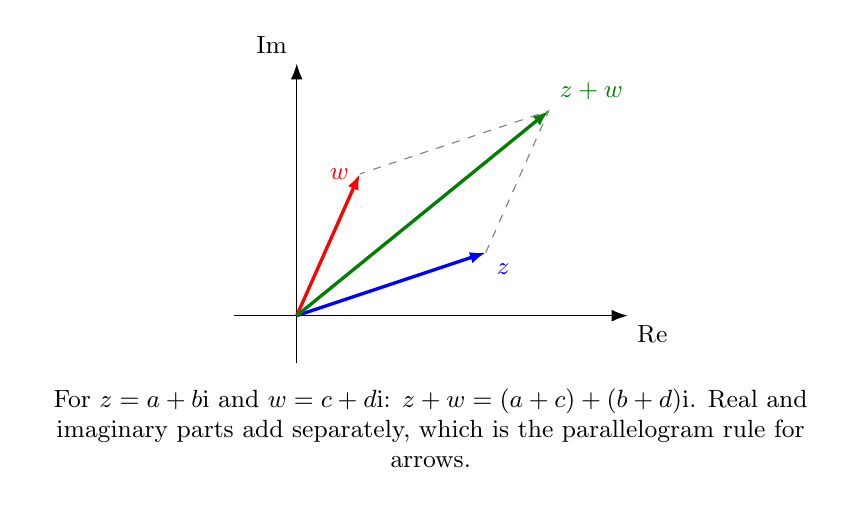
\begin{tikzpicture}[every node/.style={font=\small}, >={Latex[length=2mm]}]
	\draw[->] (-0.8,0) -- (4.2,0) node[below right] {$\mathrm{Re}$};
	\draw[->] (0,-0.6) -- (0,3.2) node[above left] {$\mathrm{Im}$};
	\draw[->, blue, very thick] (0,0) -- (2.4,0.8) node[below right] {$z$};
	\draw[->, red, very thick] (0,0) -- (0.8,1.8) node[left] {$w$};
	\draw[->, green!50!black, very thick] (0,0) -- (3.2,2.6) node[above right] {$z+w$};
	\draw[dashed, gray] (2.4,0.8) -- (3.2,2.6) -- (0.8,1.8);
	\node[anchor=north, align=flush center, text width=10cm] at (1.7,-0.8) {For $z=a+b\mathrm{i}$ and $w=c+d\mathrm{i}$: $z+w=(a+c)+(b+d)\mathrm{i}$. Real and imaginary parts add separately, which is the parallelogram rule for arrows.};
\end{tikzpicture}
\end{document}
